%\begin{Pre_Settings}
\documentclass[UTF8]{ctexart}
% \usepackage{CJK}
\usepackage{fancyhdr}
\usepackage{extramarks}
\usepackage{amsmath}
\usepackage{amssymb}
\usepackage{latexsym}
\usepackage{amsthm}
\usepackage{amsfonts}
\usepackage{tikz}
\usepackage[plain]{algorithm}
\usepackage{algpseudocode}
\usepackage{geometry}
\usepackage{graphicx}


\usepackage{subfigure}
\usepackage{booktabs}
\usepackage{indentfirst}
\usepackage{tabularx}
\usepackage{array}
\usepackage{listings}
\usepackage{xcolor}

\usepackage{calc}


% (1) choose a font that is available as T1
% for example:
\usepackage{lmodern}
% (2) specify encoding
\usepackage[T1]{fontenc}
% (3) load symbol definitions
\usepackage{textcomp}
%\end{Pre_Settings}


%\begin{Code_Settings}
\lstset{ %
language=C++,                % the language of the code
basicstyle=\footnotesize,           % the size of the fonts that are used for the code
numbers=left,                   % where to put the line-numbers
numberstyle=\tiny\color{gray},  % the style that is used for the line-numbers
stepnumber=2,                   % the step between two line-numbers. If it's 1, each line 
% will be numbered
numbersep=5pt,                  % how far the line-numbers are from the code
backgroundcolor=\color{white},      % choose the background color. You must add \usepackage{color}
showspaces=false,               % show spaces adding particular underscores
showstringspaces=false,         % underline spaces within strings
showtabs=false,                 % show tabs within strings adding particular underscores
backgroundcolor=\color[RGB]{245,245,244},
framexleftmargin=0mm,
frame=none,       % if not set, the frame-color may be changed on line-breaks within not-black text (e.g. commens (green here))
tabsize=4,                      % sets default tabsize to 2 spaces
captionpos=b,                   % sets the caption-position to bottom
breaklines=true,                % sets automatic line breaking
breakatwhitespace=false,        % sets if automatic breaks should only happen at whitespace
title=\lstname,                 % show the filename of files included with \lstinputlisting;
% also try caption instead of title
keywordstyle=\color{blue},          % keyword style
commentstyle=\color[RGB]{0,96,96},       % comment style
stringstyle=\color{orange},         % string literal style
escapeinside={\%*}{*)},            % if you want to add LaTeX within your code
morekeywords={*,...}  
}
%\end{Code_Settings}


%\begin{Passage_Settings}
\CTEXsetup[format={\Large\bfseries}]{section}

% Basic Document Settings
\topmargin=-0.45in
\evensidemargin=0in
\oddsidemargin=0in
\textwidth=6.5in
\textheight=9.0in
\headsep=0.25in

\linespread{1.1}

\pagestyle{fancy}
\lhead{\hmwkSubject}
\chead{\hmwkSemester}
\rhead{\hmwkClassNum}
\lfoot{\lastxmark} 
\cfoot{\thepage}

\renewcommand\headrulewidth{0.4pt}
\renewcommand\footrulewidth{0.4pt}
\newcolumntype{Y}{>{\centering\arraybackslash}X} 


\setlength\parindent{0pt}

\title
{
    \vspace{2in}
    \textmd{\textbf{\hmwkClass:\ \hmwkTitle}}\\
    \normalsize\vspace{0.1in}\small{Due\ on\ \hmwkDueDate\ }\\
    \vspace{1in}
    }
%\end{Passage_Settings}


%\begin{init}
\newcommand{\hmwkSemester}{2019年夏季学期}
\newcommand{\hmwkClassNum}{智能家居终端}
\newcommand{\hmwkSubject}{《电子系统设计》}
\newcommand{\chinesedash}{\rule[.7ex]{\widthof{二字}}{0.5pt}}
%\end{init}
    

%\begin{main}
\begin{document}
    
%Titlepage
\begin{titlepage}
    \begin{center}
        \phantom{Start!}
        \vspace{2in}
        \center{\zihao{-1}\textbf{TARS智能家居终端}}
        \newline
        \newline
    \rightline{\zihao{-1}\textbf{\chinesedash 电子系统设计课程报告}}
    \setlength{\baselineskip}{40pt}
    \vspace{1.5cm}
    \zihao{-2}
    \vspace{1.5cm}
    \center{
        \begin{tabular}{cl}
        组号:&  666  \\\\
        姓名:& 张雨阳、张亦弛、孙玉东\\\\
        日期:&  2019.8.30 \\\\
        \end{tabular}
        }
    \end{center}
\end{titlepage}
\pagebreak
%end_Titlepage

\section{选题背景与意义}
    \hspace{1.5em}在这个信息时代,万物互联,织成了一张无形的大网。身处其中的我们,只要说几句话、敲几下键盘,就能轻松借助物联网完成想做的事。相形之下,我们的日常生活就显得有所欠缺。基于此,我们决定制作一款智能终端(智能家居机器人终端),把这样的科技感与便捷感带进日常生活。

    \hspace{1.5em}我们智能终端的灵感来源于星际穿越中的智能机器人TARS,它将能够完成家居环境中的电器系统管理,并提供远程遥控、语音控制的双重支持,为我们的生活带来极大的便利。

\section{系统架构设计与方案比选}
    \hspace{1.5em}如图所示,整个智能终端系统有输入、处理、输出三个层次。我们提供了“语音控制”以及“远程控制”两种输入方式;“移动”、“电器控制”、“用户反馈”三种输出形式。下面一一介绍。
    \begin{figure}[H]
        \centering
        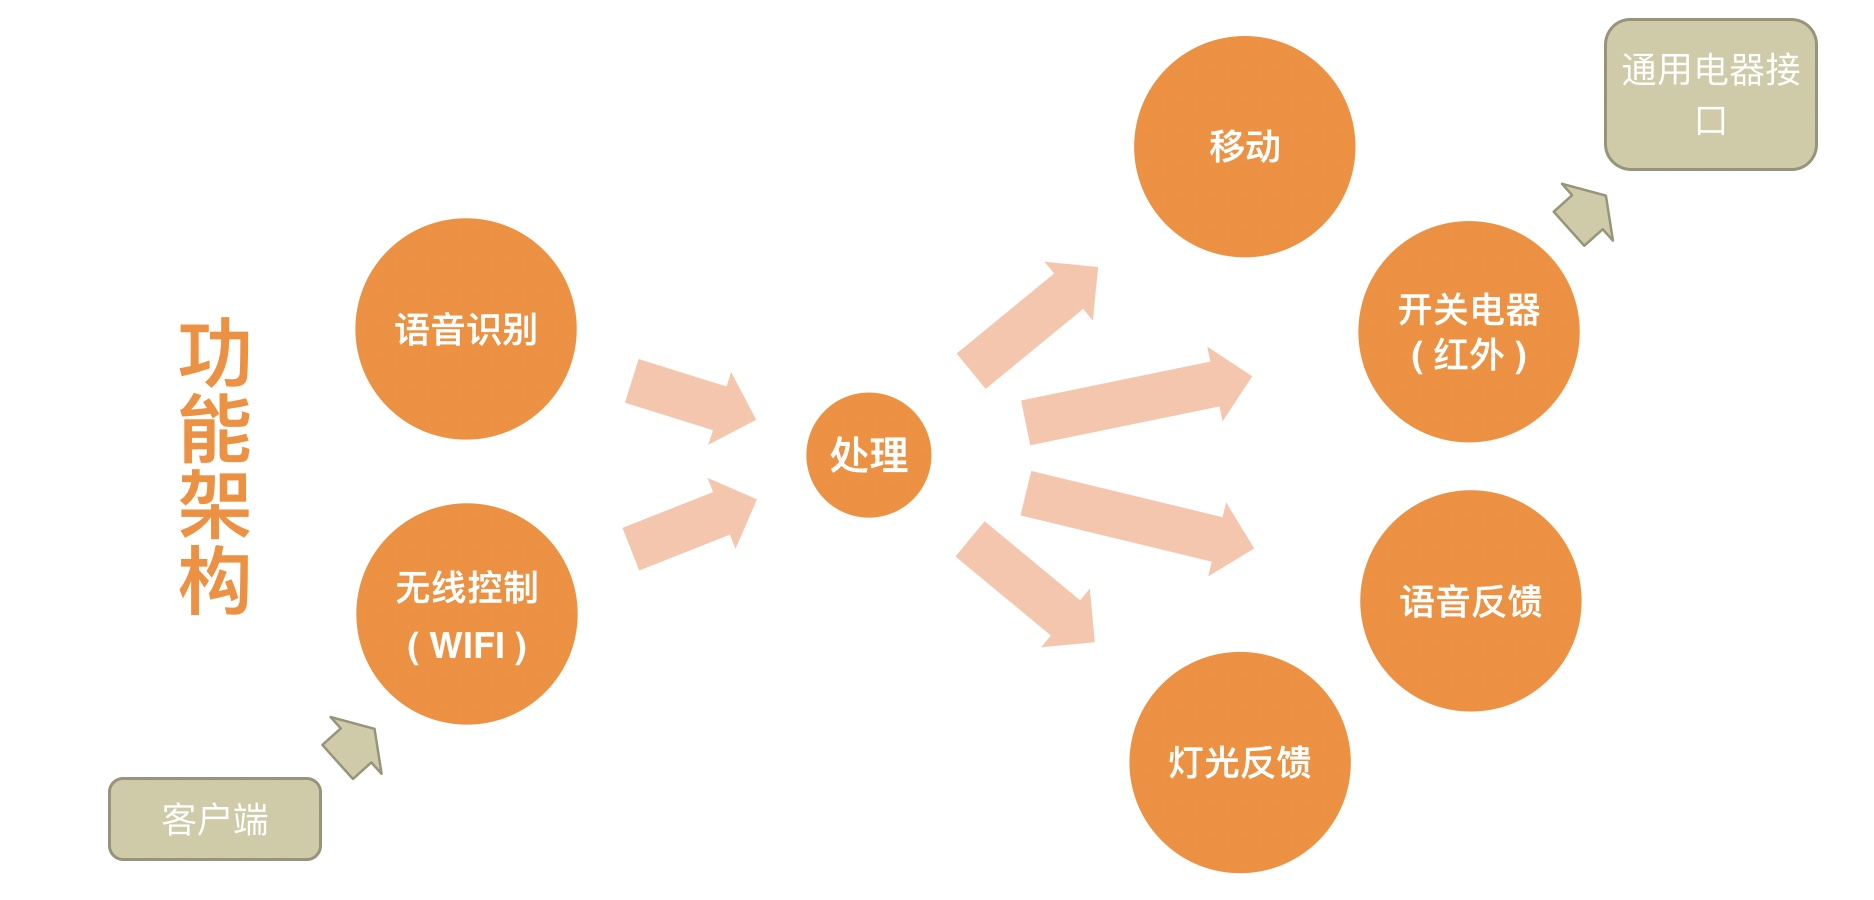
\includegraphics[width=0.4\textwidth]{./img/Structure.jpg}
    \end{figure}
    \subsection{输入}
    \subsubsection{语音控制}
    \hspace{1.5em}经过调研,我们起初准备使用LD3320语音识别模块进行识别,并搭配XFS5152语音合成模块以实现发声的功能。但由于两个模块显得冗余,加之成本过高、收货时间过晚等问题,最终选择了集成程度更高的NEWWAY语音识别模块。

    \hspace{1.5em}NEWWAY语音识别模块集成了语音识别、语音合成、播放功能,并提供了程序开发文档以及相应的IDE。利用这些硬件、软件资源,我们只需要做一些顶层开发即可实现智能终端需要的功能。

    \hspace{1.5em}于是我们设计了如下图所示的语音控制逻辑框架。此逻辑框架由五个模态组成,分别为“初始化模态”、“TARS模态”以及“睡眠模态”。
    \begin{figure}[H]
        \centering
        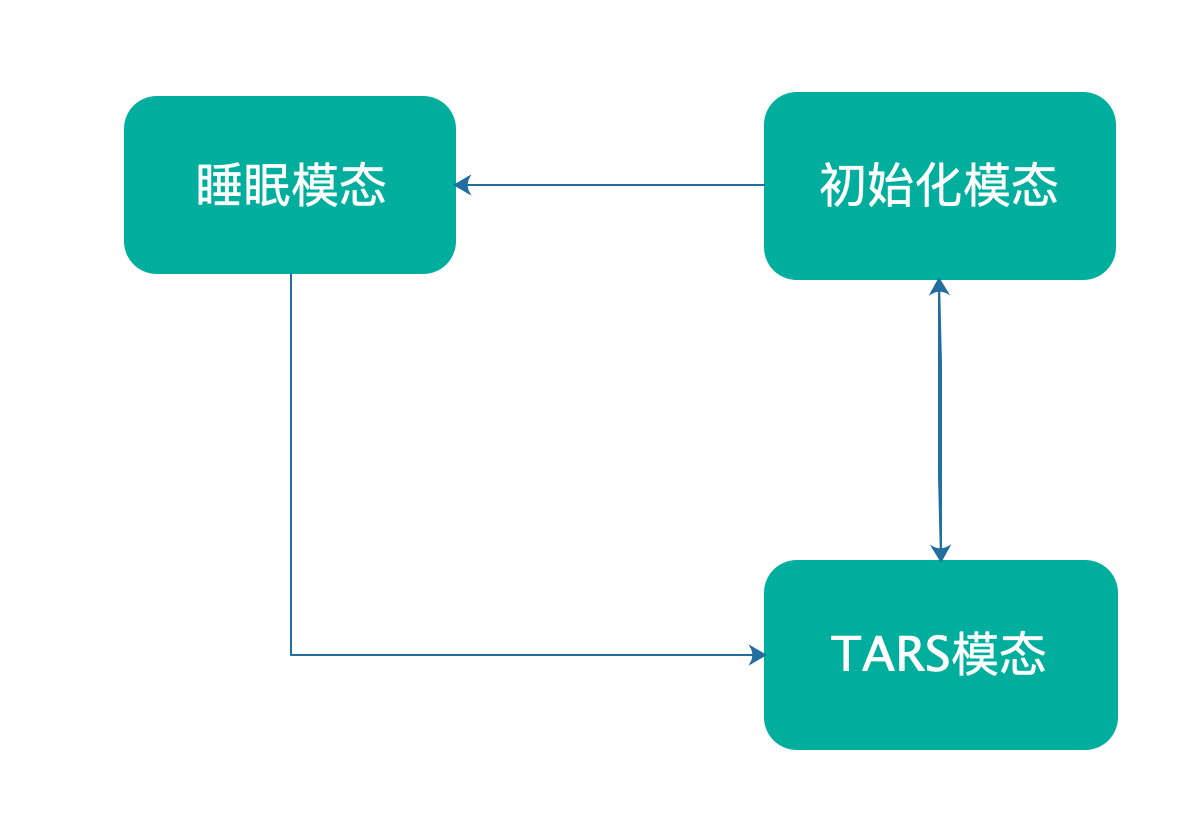
\includegraphics[width=0.4\textwidth]{./img/Mode.png}
    \end{figure}
    \hspace{1.5em}智能终端开启后即进入\textbf{“初始化模态”}。在初始化模态中,终端能够识别“TARS”和“睡眠”两个关键词并进入相应模态。如果在初始化模态中停留超过15分钟没有进行任何动作,则自动进入睡眠模态。
    
    \hspace{1.5em}进入\textbf{“TARS模态”}之后,智能终端可以识别一系列语音指令并向单片机发出消息(具体通信协议详见附件中“通信协议.pdf”):
    \begin{itemize}
        \item 行进指令
        \begin{enumerate}
            \item “前进”:向单片机发送“前进一步”的指令
            \item “后退”:向单片机发送“后退一步”的指令
        \end{enumerate}
        \item 空调控制指令:
        \begin{enumerate}
            \item “开空调”:向单片机发送“打开空调”的指令
            \item “关空调”:向单片机发送“关闭空调”的指令
            \item 温度控制指令:“空调X度”,则向单片机发送“将空调调节至X度”的指令
        \end{enumerate}
    \end{itemize}
    进入TARS模态如果超过15秒没有收到指令,则自动返回初始化模态。

    \hspace{1.5em}进入\textbf{“睡眠模态”}后,智能终端停止接收上述指令。当识别到关键词“TARS”后,重新返回TARS模态。

    \subsubsection{远程控制}
    \hspace{1.5em}远程控制有红外、蓝牙和无线控制几种选择。其中红外与蓝牙都只能提供本地的通信,不能为“人与智能终端处于异地”的场景提供解决方法。所以我们最终选择了无线控制。

    \hspace{1.5em}为了实现无线控制,我们选择了Particle Photon开发板:通过电脑端向云端发送指令,云端与Photon开发板进行通信。Photon开发板接收到指令后向主板发出信号,最终实现控制智能终端的功能。

    \hspace{1.5em}为了从电脑端与Photon顺利通信,我们设计了自己的通信协议(详见附件“通讯协议.pdf”),每条消息由指令头和指令消息构成。通过解析指令头,获取消息的接受对象、消息条数;再据此解析指令消息,最终得到所需的指令。%TODO

    \subsection{处理}
    \hspace{1.5em}所有的消息都会通过串口最终发送到主板“Arduino Mega”上,由主板根据通信协议解码后转化为相应的输出。

    \subsection{输出}
    \subsubsection{移动}
    \hspace{1.5em}智能终端最基本的输出形式就是机器人的移动,移动的说明以前进为例。
    
    \hspace{1.5em}智能终端的一次前进分为七个步骤,完全由机身上的四个舵机带动。首先抬起两条侧腿,并向前转动。转动后,侧腿前方的配重将带动智能终端向前倾倒,中心落到处在前方的两条侧腿上。此后多次重复“抬起并向前转动中间腿”的动作,最终恢复到初始角度并达到前进效果。

    \subsubsection{电器控制}
    \hspace{1.5em}智能终端共设计了两种控制用电器的方式:直接控制用电器或通过安装可控插头控制用电器。限于时间,我们只实现了前者;对前者的说明以空调控制为例。

    \hspace{1.5em}我们通过终端顶部的红外发射管向空调发送相应的红外编码,即可实现对空调的控制。

    \subsubsection{反馈}
    \hspace{1.5em}智能终端会通过“语音”、“灯光”两种形式给用户反馈。语音通过NEWWAY的语音播放功能播放;灯光由终端正面的“无限灯”展示。其中无限灯由一面“半透半返镜”以及一块平面镜组成;将一个LED灯带置于其间,即可通过光线的不断反射,形成一条灯带的无数个像,达到“无限灯”的效果。
    
    \hspace{1.5em}开机(进入前述的初始化模态)后,终端会播放语音“欢迎使用TARS”的语音,同时无限灯将发白光(如图一所示)。在进入TARS模态后,无限灯将循环发出彩色光,表示正等待指令(如图二所示)。收到指令后,智能终端将执行相应指令并使无限灯发蓝光,表示收到指令(如图三所示)。进入睡眠模式后,终端会播放语音“TARS进入睡眠模式”,并使无限灯发白光,表示进入睡眠模式。
    \begin{figure}[H]
        \begin{minipage}[htbp]{0.3\linewidth}
        \centering
        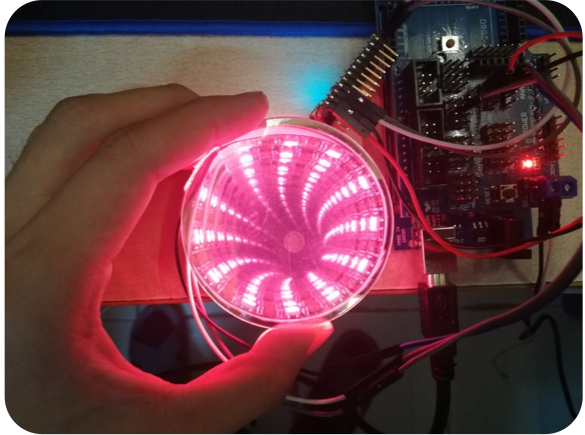
\includegraphics[width=1.7in]{./img/Light1.png}
        \caption{图一}
        \end{minipage}%
        \begin{minipage}[htbp]{0.3\linewidth}
            \centering
            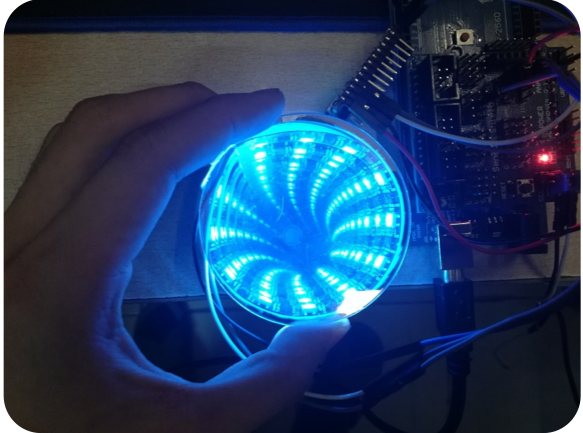
\includegraphics[width=1.7in]{./img/Light2.png}
            \caption{图二}
        \end{minipage}%    \end{figure}
        \begin{minipage}[htbp]{0.3\linewidth}
            \centering
            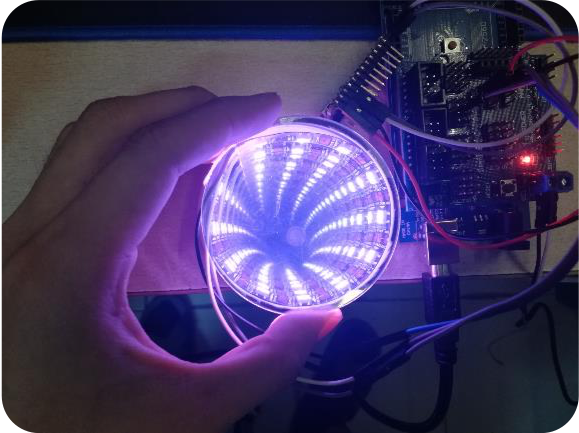
\includegraphics[width=1.7in]{./img/Light3.png}
            \caption{图三}
        \end{minipage}%
    \end{figure}
\section{程序设计}
    \hspace{1.5em}对于核心处理器Arduino Mega,考虑到Arduino对于外设中断的支持较弱,所以主要采用阻塞式面向过程程序设计。在每个循环中先尝试读取由Photon和Newway发来的协议化串口消息,并对其中的数据进行解析、处理、执行;然后考虑到LED灯带有时需要渐变或连续改变亮度与颜色,所以在主循环体中也加入了LED灯带显示的相关代码。
    \begin{lstlisting}[language={C++}]
void loop() {
    Serial1Input();

    // led display
    /* some code here */
    FastLED.show();
    FastLED.delay(1000 / UPDATES_PER_SECOND);
}
    \end{lstlisting}
    \hspace{1.5em}具体说明对数据进行处理执行的过程,我们将每个输出模块的相关代码整理成单独的库文件,通过调用其中的函数接口来执行相关操作。其中包括了红外发送、行动前进指令、行动调试模式、LED灯带变色等所有在系统架构设计章节所提到的功能。

    \hspace{1.5em}对于网路端消息分发结点Particle Photon,其代码内容即是定义处理POST请求的相关函数接口,并将POST请求中所包含的信息重新整合后通过串口发送给核心处理器Arduino Mega。

\newpage

\section{测试过程}
    \subsection{机械结构调试}
    \hspace{1.5em}在拼装机械结构的过程中,我们发现了一系列问题。对于侧腿左右摇晃的问题,我们增加了齿条挡板,控制了齿条的晃动,进而减小了侧腿晃动幅度;对于侧腿质量过大导致舵机与齿轮接口被磨损的问题,我们将舵机型号更换为“MG996R”(接口为金属材质),其接口材料的耐磨性有效的解决了材料磨损问题。此外,我们前期考虑不周,没有为终端正面的“无限灯”、背面的“电源开关”留出空间,最后重新切割相应模板解决了问题。

    \subsection{前进动作的调试}
    \hspace{1.5em}如上所述,一次前进主要为抬腿前倾、收腿归位两大部分,共分为七个小步骤。我们通过云端给系统中的Particle Photon发送debug指令,不断调节侧腿的上升距离、旋转角度参数,最终得到理想的结果。
    \hspace{1.5em}起初在相对光滑的地面上,机器人在收腿归位时会因动量守恒而无法前进,导致每一步前进距离过短。而在较粗糙的地面上则因阻力过大而几乎无法收腿。我们在前腿上增加了四块配重,使重心偏向前,增大了侧腿接触面的摩擦力,最终实现了正常步幅(每步约30cm)的前进。
    \begin{figure}[H]
        \begin{minipage}[htbp]{0.5\linewidth}
        \centering
        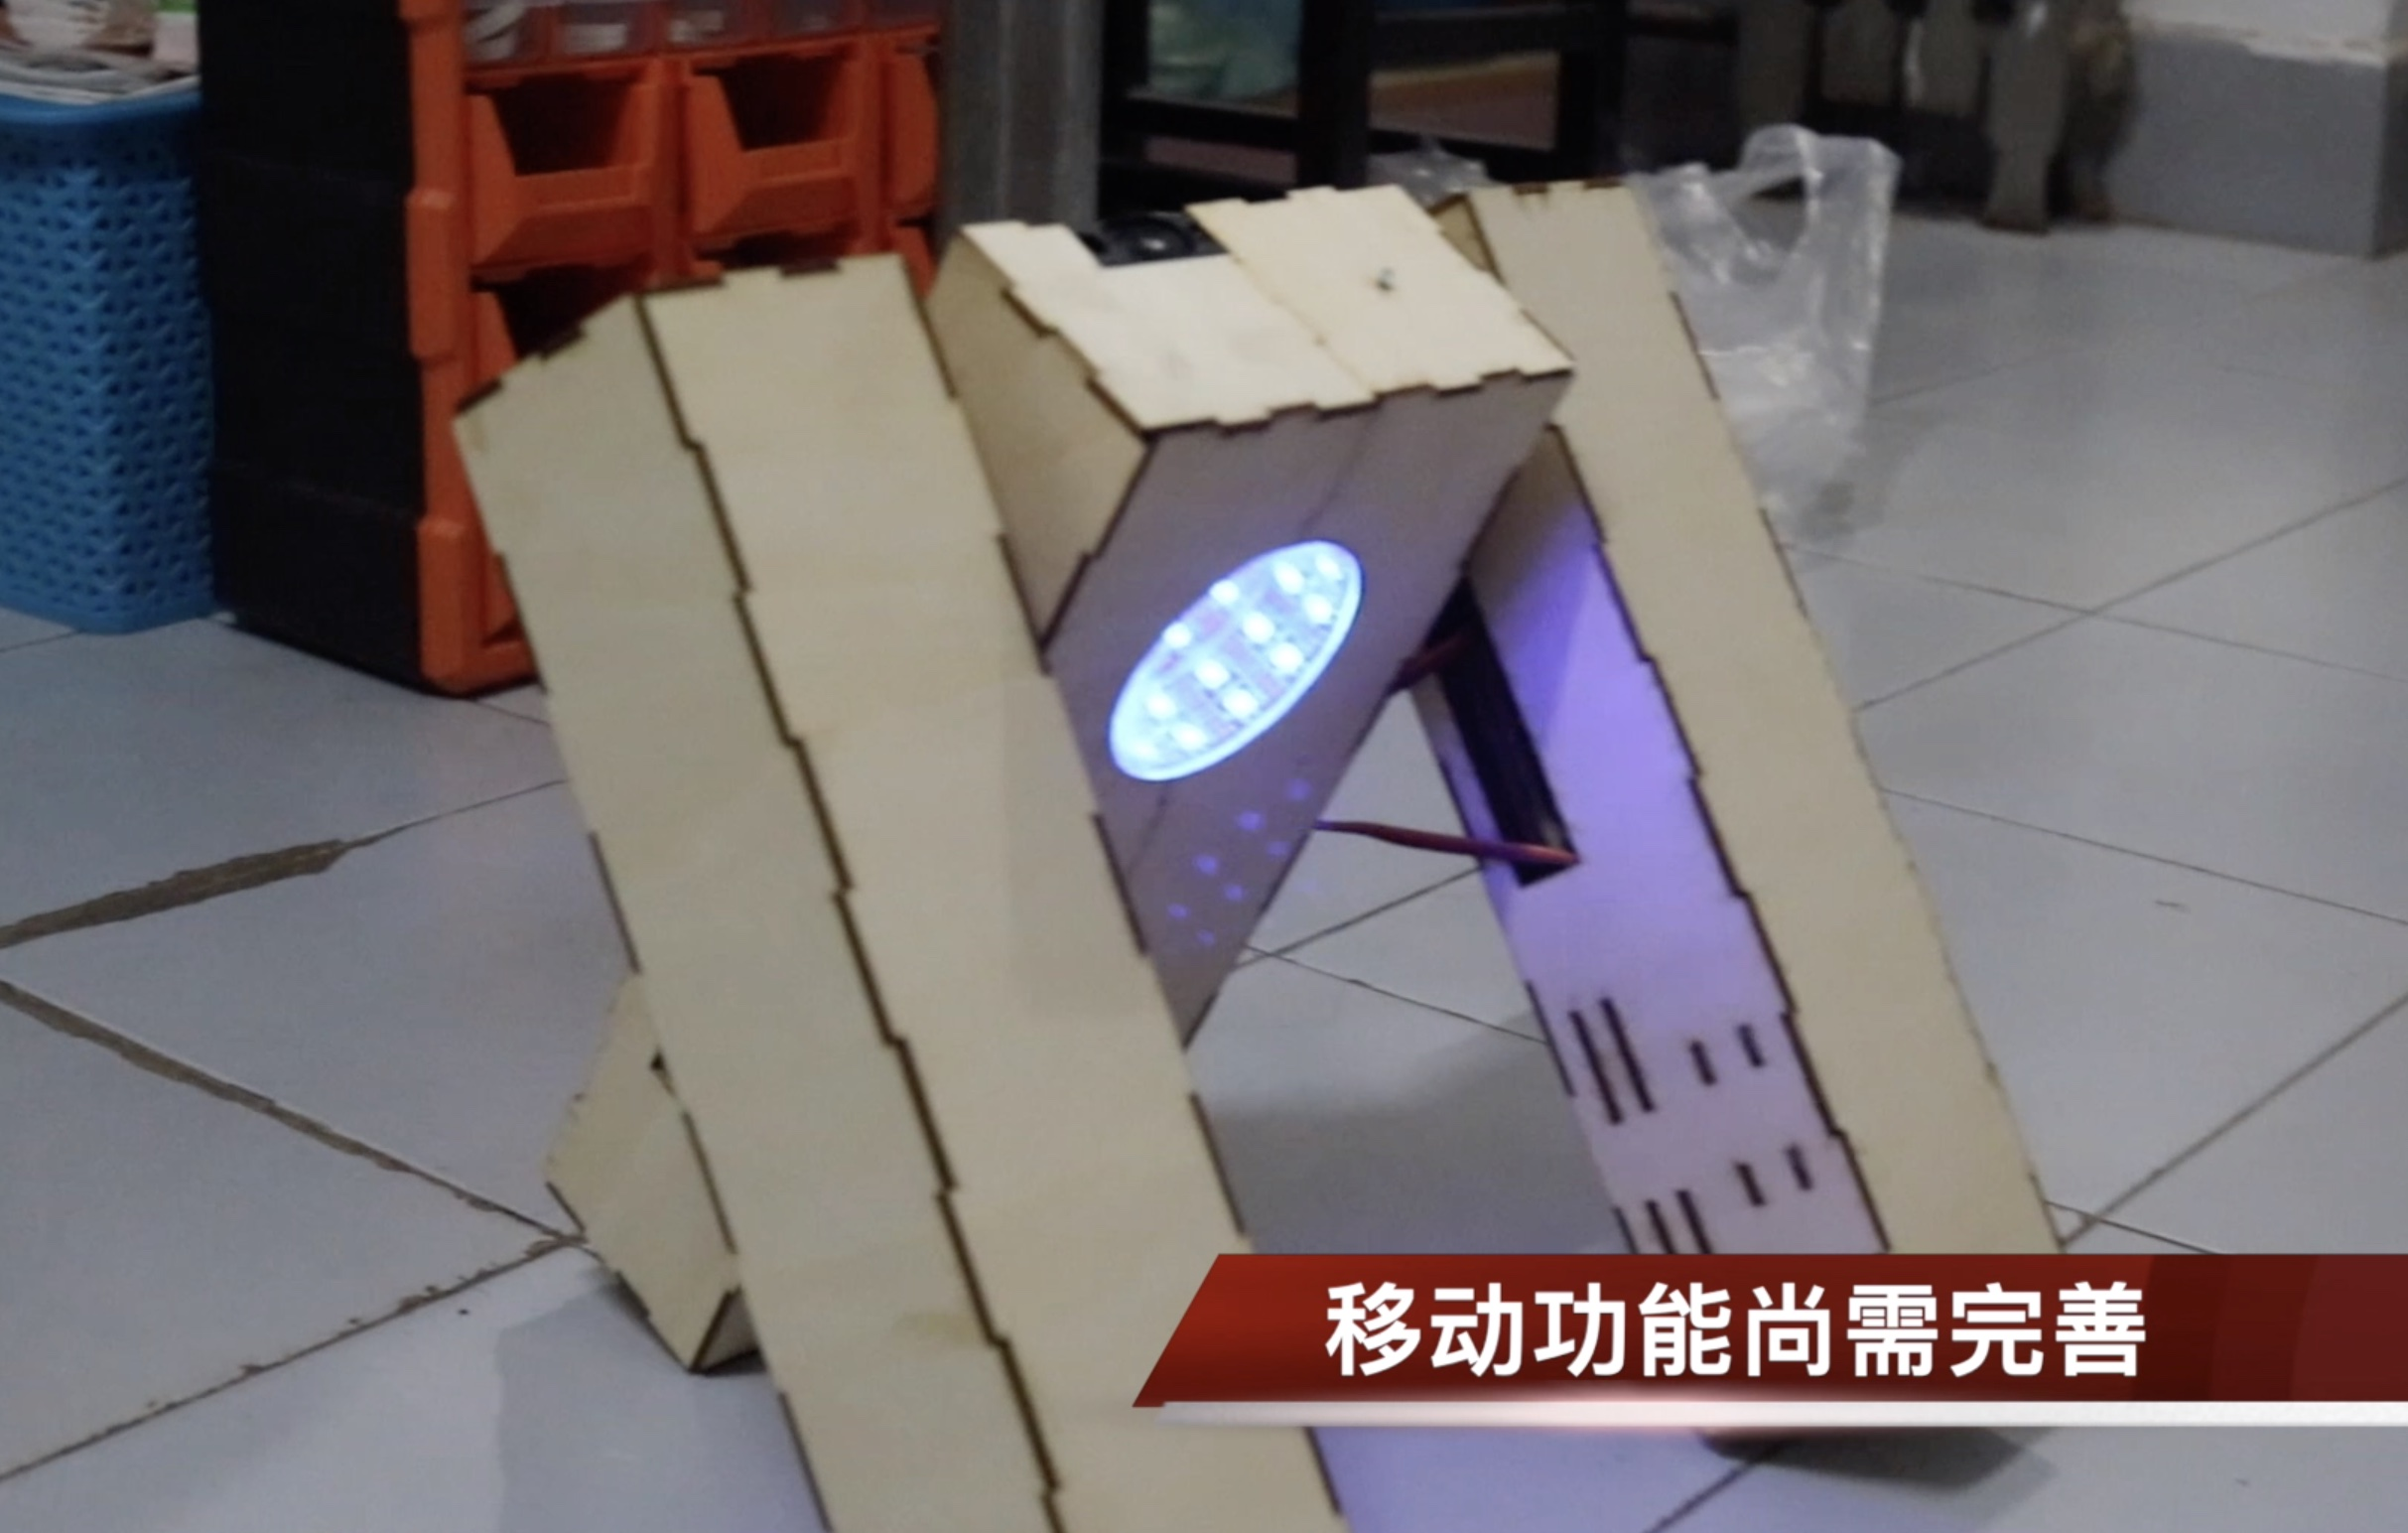
\includegraphics[width=2.2in]{./img/ForwardOld.jpg}
        \caption{改进前}
        \end{minipage}%
        \begin{minipage}[htbp]{0.5\linewidth}
        \centering
        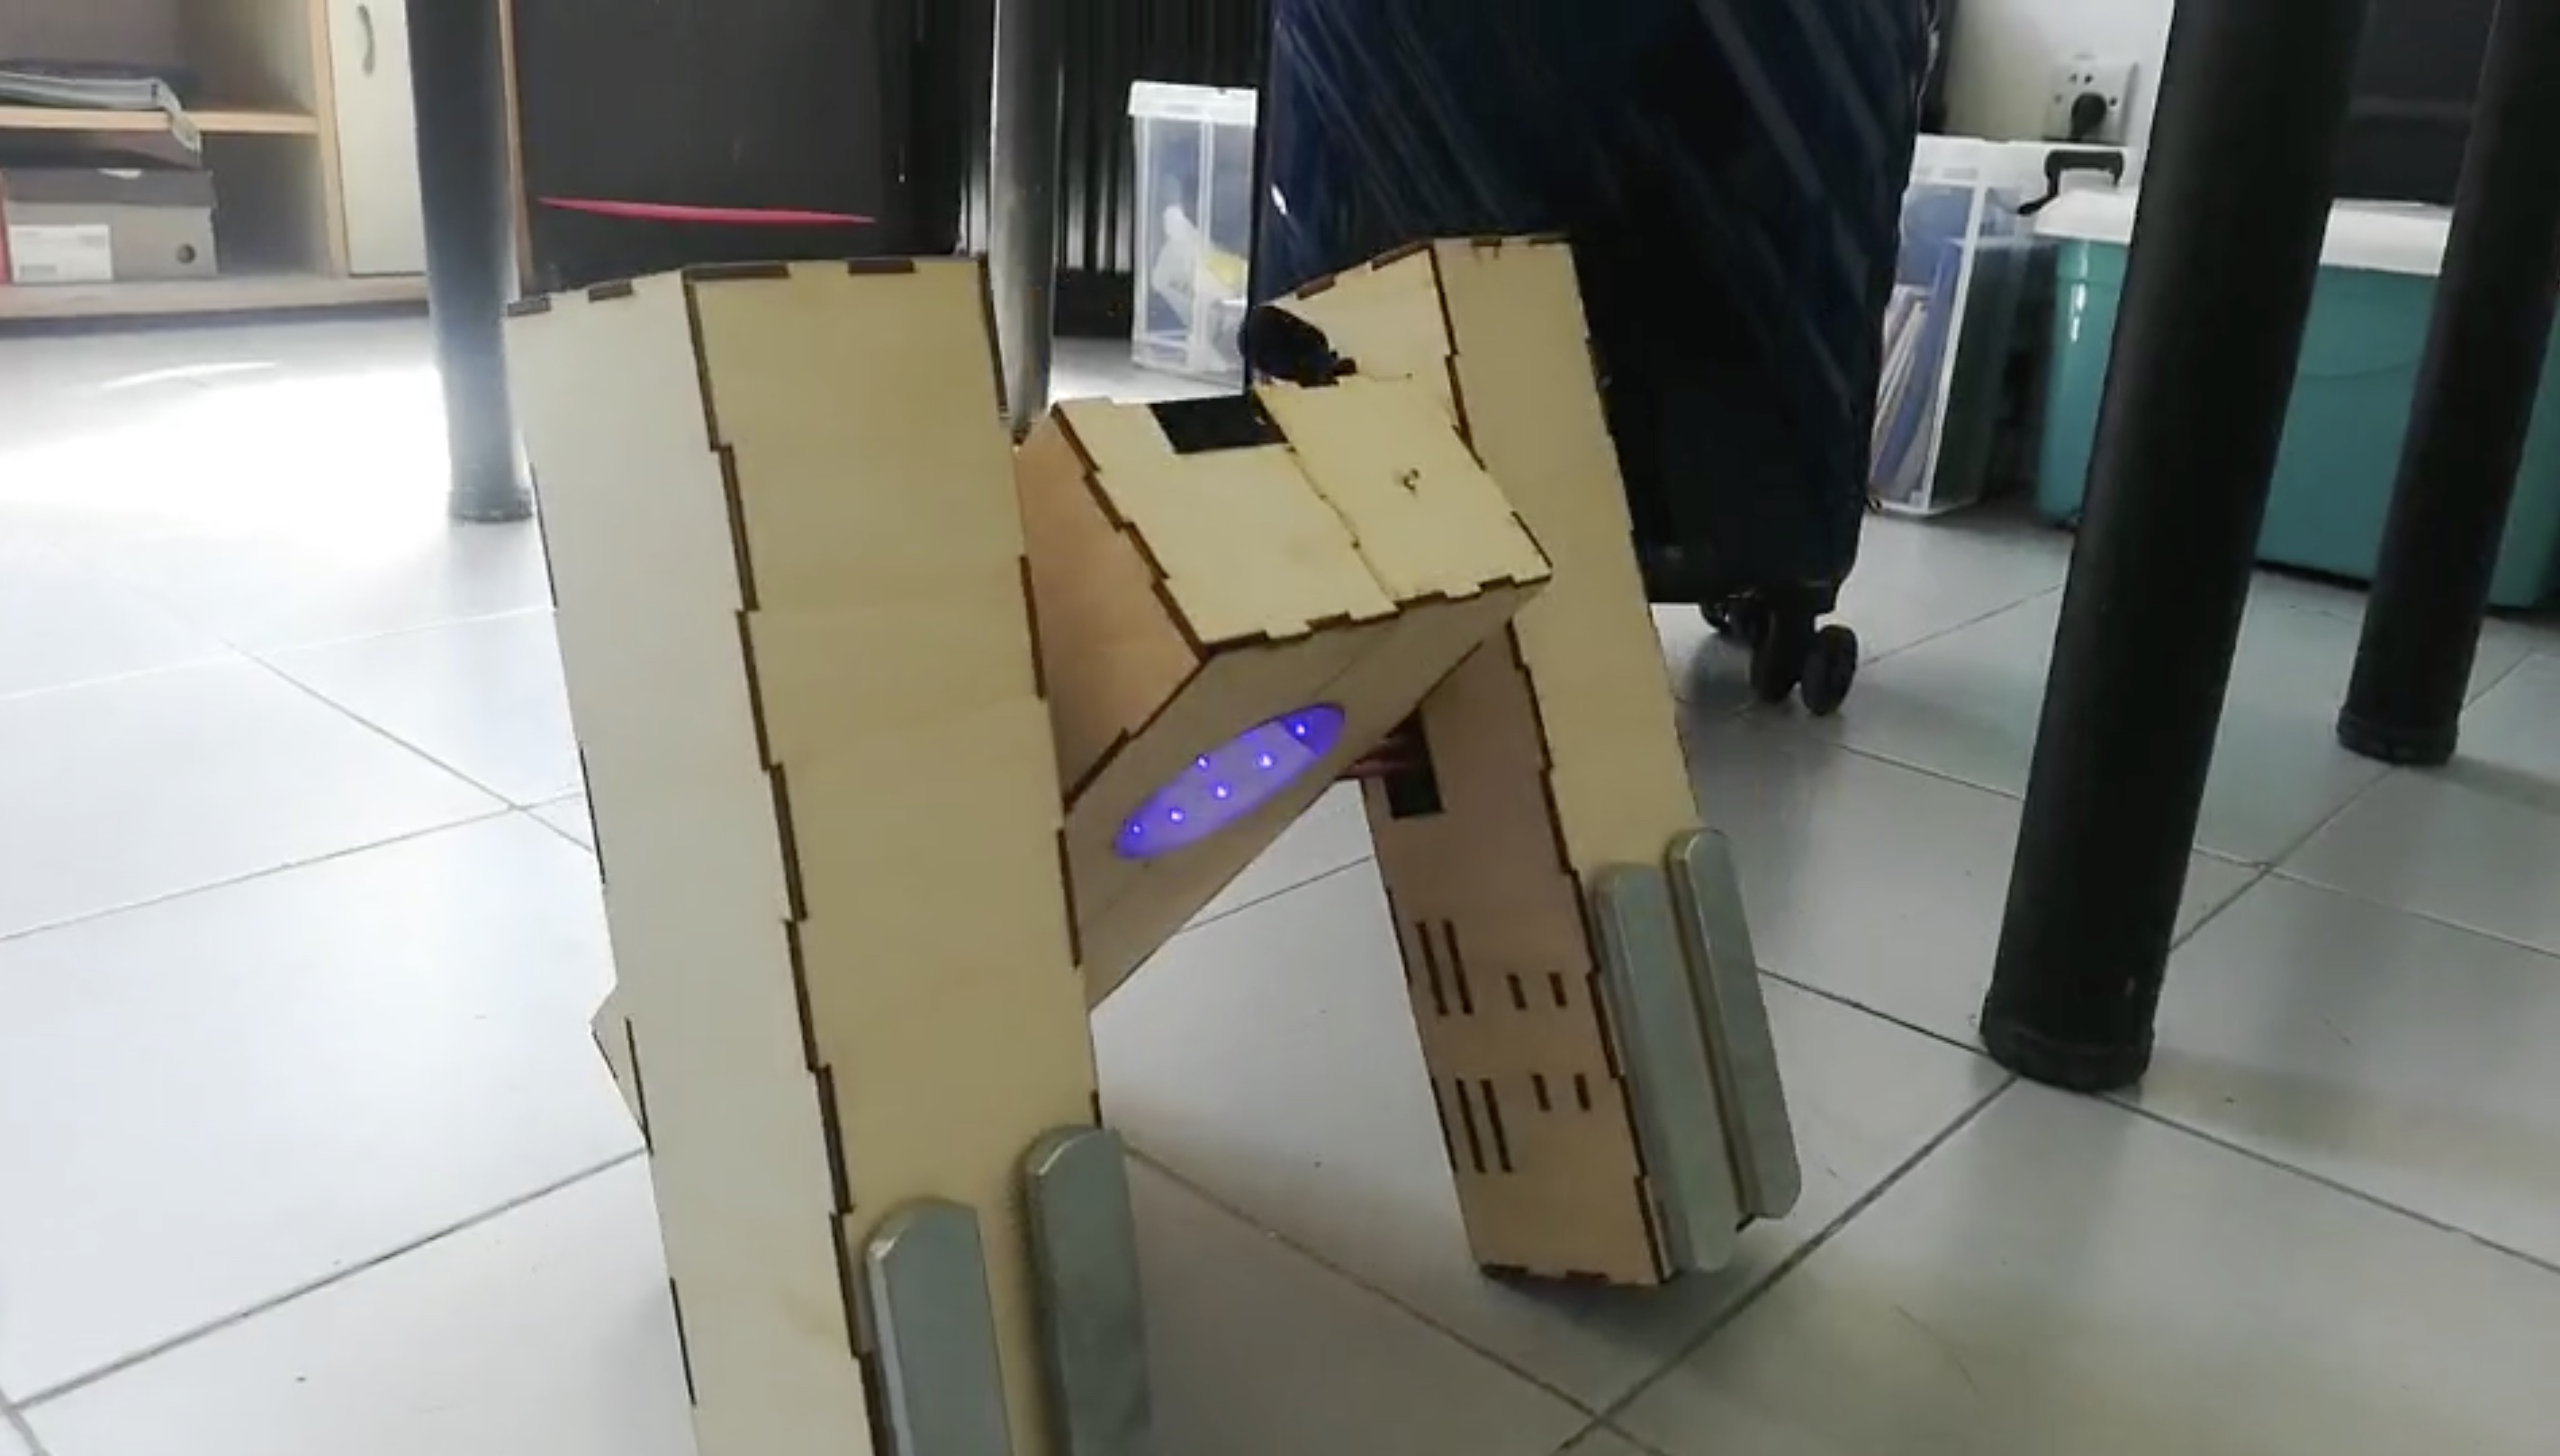
\includegraphics[width=2.2in]{./img/ForwardNew.jpg}
        \caption{改进后}
        \end{minipage}
    \end{figure}

    \subsection{红外控制的调试}
    \hspace{1.5em}我们先通过红外接收管,接收空调遥控器发出的红外编码。通过逐条比较,分析出编码与指令的关系(如温度控制位、模式控制位的位置)。最后根据这些规律得到我们需要的红外编码(打开空调、关闭空调、设置温度为27度等)。

    \hspace{1.5em}之后将得到的编码通过红外发射管向空调输出时,发现信号不起作用。通过深入分析,发现每条指令中除了数据位还包含了校验位。由于缺乏相应的分析知识,我们放弃了自行编码,最终选择手动记录每条指令对应的红外编码。将原始编码通过发射管发出后生效,测试成功。

    \subsection{电路修正}
    \hspace{1.5em}我们电路搭建完成后,进行电路测试却发现NEWWAY语音识别模块通过串口发送的消息无法被检测,只能收到Photon模块的串口消息。
    \hspace{1.5em}我们猜测可能是因为Photon内部的上下拉过强,导致NEWWAY串口信号被屏蔽。于是我们在Photon的TX端口串联了200R的限流电阻,并再次进行收发测试。此时发现两边数据都能被正常接收。修正成功。

\newpage

\section{应用前景}
\hspace{1.5em}在这个讲求万物智能互联的时代,用物联网的思想和技术,将生活中的设备进行智能化统一管理是一个符合发展潮流的方向。它可以被用在家庭中,作为一个远程控制家具的终端,即使出门在外也可以监控家中的情况,或者在回家之前先将室内环境调节到最佳状态。它也可以被用于实验室、活动室,实现对器件分发的记录,以及设备使用情况的管控。可移动的功能更给它在大型室内环境中掌控全局的能力。

\section{未来展望}
\hspace{1.5em}我们在项目的制作与设计过程中,布置了许多可拓展、易拓展的接口。例如基于wifi的无限操控使得以后增加网络客户端成为可能;红外遥控这种普遍的遥控形式使得各种常用家用电器(例如电视、空调等)都可以成为目标控制对象,并且可以自行设计受红外控制的插座,实现一键通电断电。最重要的是,这些可拓展的功能并不需要对终端本体进行大幅度改动,所以很大成度的保护了它的独立性。

\hspace{1.5em}除了新功能模块的加入,现有功能也有一些改进与优化的空间。在机械方面,外观的调整(比例、涂装等)是一个重要的方向;在硬件电路方面,我们希望能将冗余的几块带处理器的模块替换为更简单的模块,比如用esp8266代替Photon,或者进一步考虑如果使用体量更轻的语音识别与人声合成的解决方案,都是我们十分希望能在将来完成的改进。还有一些小细节,例如布线、红外发射功率、系统的鲁棒性等等,都有进一步提升的空间。



\end{document}
%\end{main}